%%%%%%%%%%%%%%%%%%%%%%%%%%%%%%%%%%%%%
%                                   %
% Compile with XeLaTeX and biber    %
%                                   %
% Questions or comments:            %
%                                   %
% joshua dot mcneill at uga dot edu %
%                                   %
%%%%%%%%%%%%%%%%%%%%%%%%%%%%%%%%%%%%%

\documentclass{beamer}
  % Read in standard preamble (cosmetic stuff)
  %%%%%%%%%%%%%%%%%%%%%%%%%%%%%%%%%%%%%%%%%%%%%%%%%%%%%%%%%%%%%%%%
% This is a standard preamble used in for all slide documents. %
% It basically contains cosmetic settings.                     %
%                                                              %
% Joshua McNeill                                               %
% joshua dot mcneill at uga dot edu                            %
%%%%%%%%%%%%%%%%%%%%%%%%%%%%%%%%%%%%%%%%%%%%%%%%%%%%%%%%%%%%%%%%

% Beamer settings
% \usetheme{Berkeley}
\usetheme{CambridgeUS}
% \usecolortheme{dove}
% \usecolortheme{rose}
\usecolortheme{seagull}
\usefonttheme{professionalfonts}
\usefonttheme{serif}
\setbeamertemplate{bibliography item}{}

% Packages and settings
\usepackage{fontspec}
  \setmainfont{Charis SIL}
\usepackage{hyperref}
  \hypersetup{colorlinks=true,
              allcolors=blue}
\usepackage{graphicx}
  \graphicspath{{../../figures/}}
\usepackage[normalem]{ulem}
\usepackage{enumerate}

% Document information
\author{M. McNeill}
\title[FREN2001]{Français 2001}
\institute{\url{joshua.mcneill@uga.edu}}
\date{}

%% Custom commands
% Lexical items
\newcommand{\lexi}[1]{\textit{#1}}
% Gloss
\newcommand{\gloss}[1]{`#1'}
\newcommand{\tinygloss}[1]{{\tiny`#1'}}
% Orthographic representations
\newcommand{\orth}[1]{$\langle$#1$\rangle$}
% Utterances (pragmatics)
\newcommand{\uttr}[1]{`#1'}
% Sentences (pragmatics)
\newcommand{\sent}[1]{\textit{#1}}
% Base dir for definitions
\newcommand{\defs}{../definitions}


  % Packages and settings

  % Document information
  \subtitle[Traits et questions]{Encore les traits et les questions}

\begin{document}
  % Read in the standard intro slides (title page and table of contents)
  \begin{frame}
    \titlepage
    \tiny{Office: % Basically a variable for office hours location
Gilbert 121\\
          Office hours: % Basically a variable for office hours
 lundi, mercredi, vendredi 10:10--11:10
}
  \end{frame}

  \begin{frame}{Annonces}
    \begin{itemize}
      \item Le devoir 2 est à rendre le 22 septembre.
      \item[] \tinygloss{Homework 2 is due September 22nd.}
    \end{itemize}
  \end{frame}

  \begin{frame}{}
    \begin{center}
      \Large Quiz
    \end{center}
  \end{frame}

  \begin{frame}{C'est un homme ou une femme?}
    \begin{center}
      Camille est \underline{\uncover<2->{amusan\sout{t}}} \\
      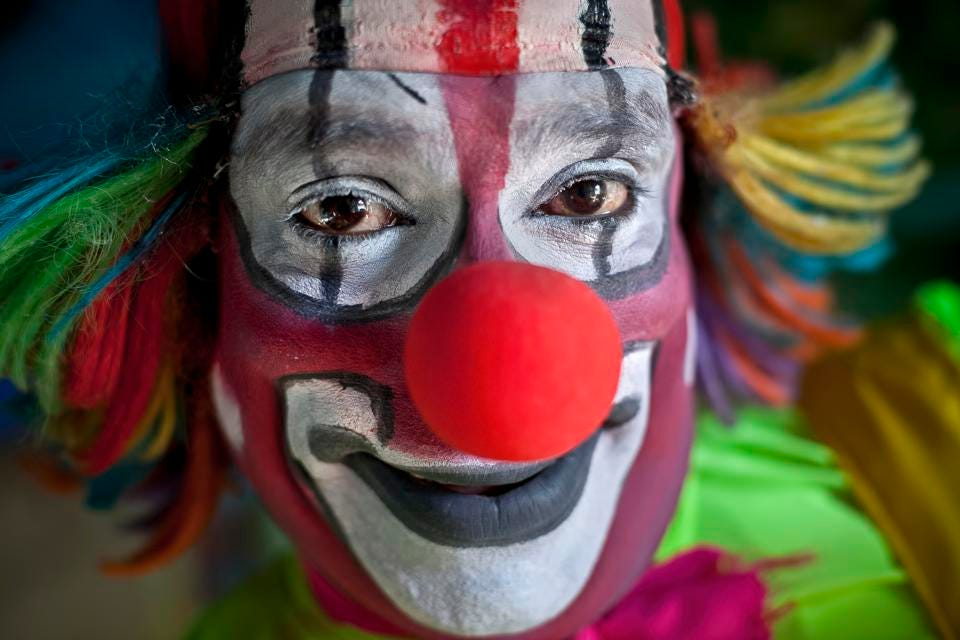
\includegraphics[scale=0.25]{clown.jpg}
    \end{center}
  \end{frame}

  \begin{frame}{C'est un homme ou une femme?}
    \begin{center}
      Sacha est \underline{\uncover<2->{gro\sout{s}}} \\
      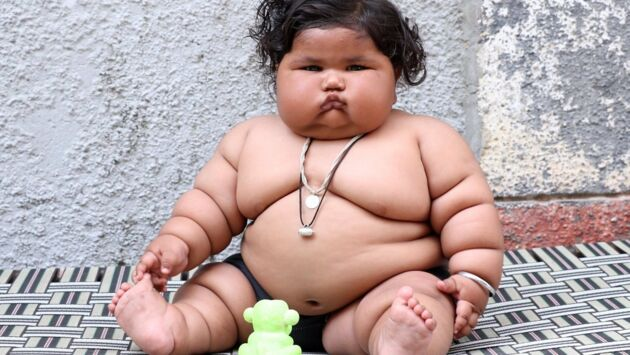
\includegraphics[scale=0.45]{gros.jpg}
    \end{center}
  \end{frame}

  \begin{frame}{C'est un homme ou une femme?}
    \begin{center}
      Éloi est \underline{\uncover<2->{intelligen\alert{te}}} \\
      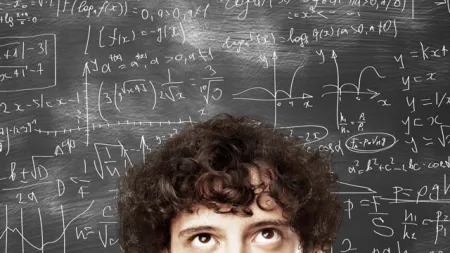
\includegraphics[scale=0.6]{intelligente.jpg}
    \end{center}
  \end{frame}

  \begin{frame}{C'est un homme ou une femme?}
    \begin{center}
      Laurence est \underline{\uncover<2->{ambitieu\alert{se}}} \\
      
\includegraphics[scale=0.35]{ambitieuse.jpg}
    \end{center}
  \end{frame}

  \begin{frame}{C'est un homme ou une femme?}
    \begin{center}
      Patrice est \underline{\uncover<2->{blon\sout{d}}} \\
      
\includegraphics[scale=0.75]{blond.jpg}
    \end{center}
  \end{frame}

  \begin{frame}{C'est un homme ou une femme?}
    \begin{center}
      Ange est \underline{\uncover<2->{bru\alert{ne}}} \\
      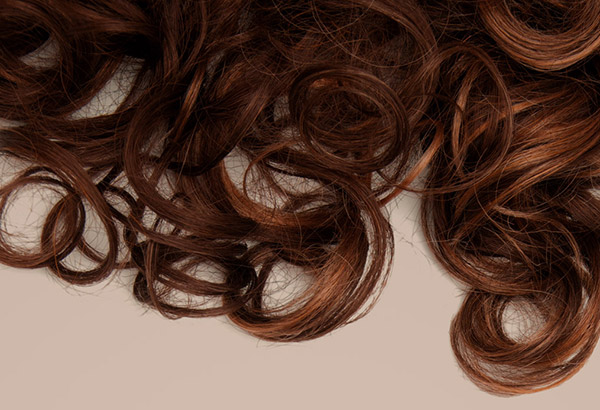
\includegraphics[scale=0.35]{brune.jpg}
    \end{center}
  \end{frame}

  \begin{frame}{Des traits opposés}
    Tes amis sont...
    \begin{enumerate}
      \item âgés $\to$ \underline{\uncover<2->{jeunes}}
      \item égoïstes $\to$ \underline{\uncover<3->{généreux}}
      \item bêtes $\to$ \underline{\uncover<4->{intelligents}}
      \item sédentaires $\to$ \underline{\uncover<5->{énergiques}}
      \item paresseux $\to$ \underline{\uncover<6->{ambitieux}}
      \item minces $\to$ \underline{\uncover<7->{gros}}
      \item mal habillés $\to$ \underline{\uncover<8->{élégants}}
      \item laids $\to$ \underline{\uncover<9->{beaux}}
    \end{enumerate}
  \end{frame}

  \begin{frame}{Dessinons la famille}
    \begin{columns}
      \column{0.5\textwidth}
        Décris une femme dans ta famille pour qu'un/e partenaire la dessine.
        Utilise le nouveau vocabulaire, et sois aussi descriptif que possible. \\
        \tinygloss{Describe a woman in your family for a partner to draw her.
        Use the new vocabulary, and be as descriptive as possible.}
      \column{0.25\textwidth}
        \tiny
        Elle est...
        \begin{enumerate}
          \item âgée
          \item belle
          \item blonde
          \item brune
          \item châtain
          \item de taille moyenne
          \item d'un certain âge
          \item élégante
          \item forte
          \item grande
          \item grosse
          \item jeune
          \item jolie
          \item laide
          \item maigre
          \item mal habillée
          \item mince
          \item petite
          \item rousse
        \end{enumerate}
      \column{0.25\textwidth}
        \tiny
        % \begin{enumerate}
          
        % \end{enumerate}
        Elle a les yeux...
        \begin{enumerate}
          \setcounter{enumi}{19}
          \item bleus
          \item marron
          \item noirs
          \item noisette
          \item verts
        \end{enumerate}
        Elle a les cheveux...
        \begin{enumerate}
          \setcounter{enumi}{24}
          \item blonds
          \item bouclés
          \item bruns
          \item châtains
          \item courts
          \item frisés
          \item gris
          \item longs
          \item noirs
          \item raides
          \item roux
        \end{enumerate}
    \end{columns}
  \end{frame}

  \begin{frame}{Écrivons}
    \begin{itemize}
      \item Rendez-moi les dessins.
      \item[] \tinygloss{Turn in your drawings.}
      \item<2-> Écrivez une description du dessin que vous avez reçu par des phrases complètes.
      \item<2->[] \tinygloss{Write a description of the drawing you received using complete sentences.}
    \end{itemize}
  \end{frame}

  \begin{frame}{}
    \begin{center}
      \Large Questions?
    \end{center}
  \end{frame}
\end{document}
